\documentclass[12pt,a4]{article}
\usepackage[left=1.8cm,right=1.8cm,top=32mm,columnsep=20pt]{geometry}

\usepackage[utf8]{inputenc} %Formato de codificación
\usepackage[spanish, es-tabla, es-nodecimaldot]{babel}
\usepackage{amsmath} %paquete para escribir ecuaciones matemáticas
\usepackage{float} %Para posicionar figuras
\usepackage{graphicx} %Para poder poner figuras
\usepackage{tikz}
\usetikzlibrary{positioning}
\usetikzlibrary{shapes.geometric, decorations.pathreplacing}

\title{Analisis movimiento de un pendulo}
\author{Francisco Carruthers, Facundo Firpo y Joel Jablonski\\ [2mm]
\small \texttt{\{fcarruthers, ffirpo, jjablonski\}@udesa.edu.ar}\\
\small Fisica I, tutorial Vinograd}
\date{2do Semestre 2024}


\begin{document}

\maketitle

\begin{abstract}
    Pendulo
\end{abstract}

\section{Introduccion}

\begin{equation}
    T = 2 \pi \sqrt{\frac{L}{g}}
    \label{eq:periodo}
\end{equation}

\begin{equation}
    \omega = \frac{1}{T}
    \label{eq:omega}
\end{equation}

Vamos a ver como modificar el angulo inicial, la longitud de la soga y la masa de la bolita afectan el periodo del movimiento. Viendo la ecuacion \ref{eq:periodo} podemos ver que el periodo es independiente del angulo inicial y a la masa de la bolita. Sin embargo, si depende de la longitud de la soga. 

De los datos obtenidos podemos encontrar una gravedad real del experimento, la cual es una modificacion de la conocida $g = 9.8 m/s^2$. Hay un cambio en la gravedad debido a la friccion del aire, la cual afecta el movimiento de la bolita y que ignoramos en este analisis.

De la ecuacion \ref{eq:periodo} podemos despejar la gravedad:

\begin{equation}
    g = \frac{4 \pi^2 L}{T^2}
    \label{eq:gravedad}
\end{equation}

Usando como datos $L = 42.0 \pm 0.1 cm$ y $T = 1.335 \pm 0.001 s$ obtenemos una gravedad de $g_{efectiva} = 9.30 \pm 0.03 m/s^2$.

\section{Practica experimental}

\begin{figure}[H]
    \centering
    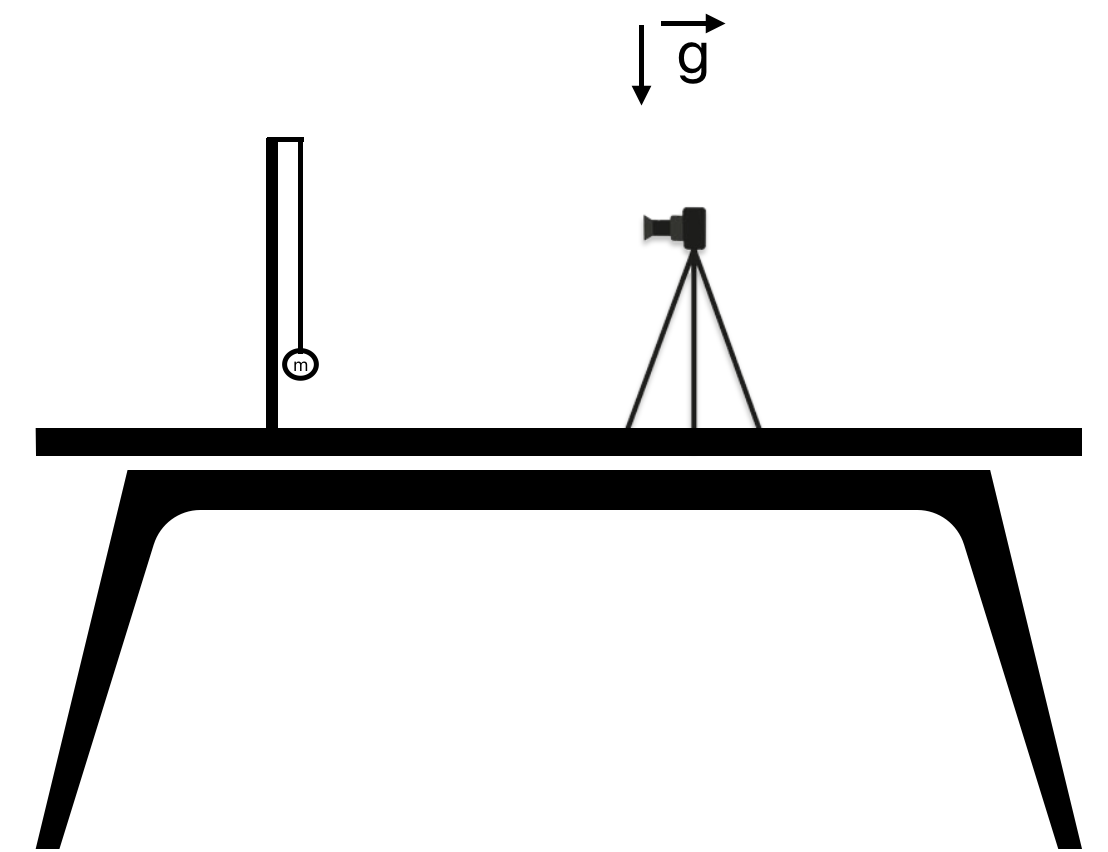
\includegraphics[width=0.6\linewidth]{esquema.png}
    \caption{Esquema del experimento}   
    \label{fig:esquema}
\end{figure}

Los errores que tuvimos en cuenta fueron los siguientes:

\begin{itemize}
    \item Error en la medicion del largo de la soga: $\pm 0.1 cm$
    \item Error en la medicion del angulo inicial: $\pm 1$
    \item Error en la posicion de la bolita: $\pm 1 cm$ (radio de la bolita)
\end{itemize}

\section{Seguimiento de la trayectoria}

Usamos la aplicacion de Tracker %\href{https://physlets.org/tracker/}{Tracker}

\section{Resultados}

Para los distintos angulos iniciales se obtuvieron los siguientes resultados:

\begin{figure}[H]
    \centering
    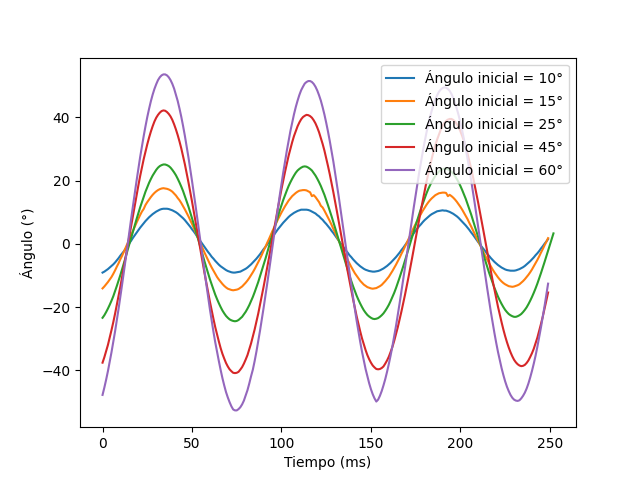
\includegraphics[width=0.6\linewidth]{angulos.png}
    \caption{Posicion de la masa en funcion del tiempo para distintos angulos iniciales}
    \label{fig:angulos}
\end{figure}

Se puede observar como la amplitud del movimiento no afecta la frecuencia del mismo. 

\begin{figure}[H]
    \centering
    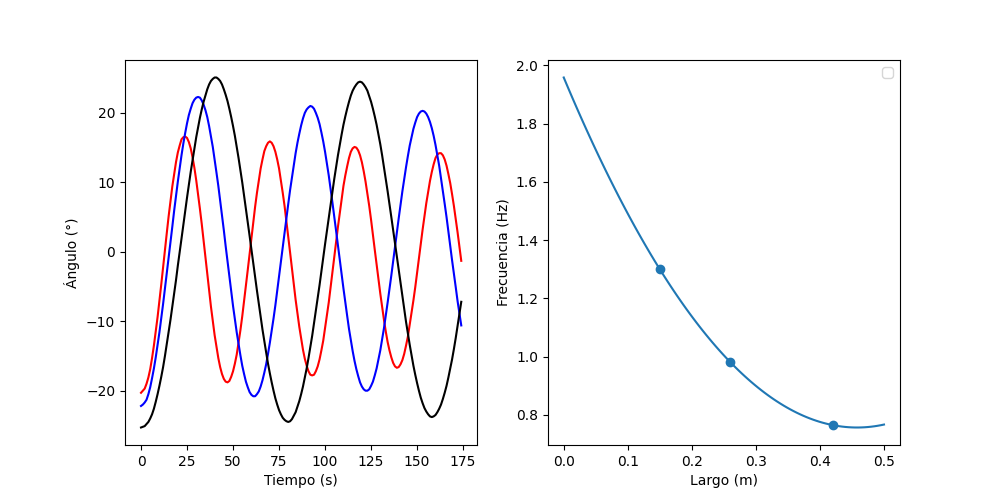
\includegraphics[width=0.6\linewidth]{largo.png}
    \caption{Posicion de la masa en funcion del tiempo para distintos largos de soga}
    \label{fig:largo}
\end{figure}

Se puede observar como el largo de la soga afecta la frecuencia del movimiento. A mayor largo, menor frecuencia. Esto se debe a que la bolita recorre una mayor distancia. Sabemos que la longitud de arco esta defenida como $d = r \theta$, por lo que a mayor longitud de soga, mayor longitud de arco recorre la bolita.

\begin{figure}[H]
    \centering
    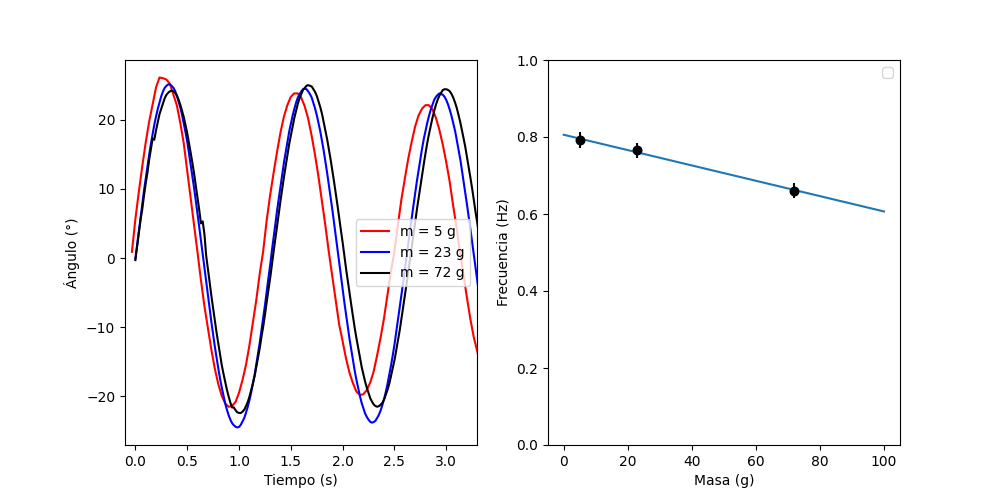
\includegraphics[width=0.6\linewidth]{peso.png}
    \caption{Posicion de la masa en funcion del tiempo para distintas masas}
    \label{fig:masa}
\end{figure}

Se puede observar como la masa de la bolita no afecta la frecuencia del movimiento excepto cuando la masa es chica. Esto se debe a en el experimento la soga no es perfectamente rigida, por lo que, al tener poca masa, el movimiento de la soga se deforma.

\end{document}